\subsection{Временное разрешение}\label{section:TimeRes}

В проведённых пучковых тестах имеют место два типа событий, в которых регистрируются несколько практически одновременно испущенных фотонов. Первый тип --- это вспышка лазера, длительность которой $\approx$40~пс, т.е. на порядок меньше разброса времени прохождения сигнала через МА~ФЭУ. Второй тип --- черенковские кольца. Разброс времени прихода фотонов на МА~ФЭУ может достигать 100~пс для колец и 70~пс для вспышек лазера, что определяется в первую очередь наклоном плоскости в которой расположены фотокатоды. Анализ таких событий позволяет охарактеризовать временное разрешение всей системы считывания, начиная от окна МА~ФЭУ и кончая формированием отметок времени. Временное разрешение одного канала определяется разбросом зарегистрированных временных отметок относительно времени прилёта фотона при многократных измерениях. Поскольку точное время прилёта фотона измерить нельзя, нам приходится исследовать разброс разностей временных отметок в паре каналов при регистрации одновременно пришедших фотонов. Временные отметки в каждом из каналов подвержены независимым флуктуациям по одинаковому закону, следовательно, измеренная ширина распределения будет в~$\sqrt 2$~раз больше, чем временное разрешение каждого канала.
%На \figref{fig:TimeRes} показано типичное распределение разностей временных отметок, принадлежащих одной вспышке лазера,
После применения коррекций задержек и калибровки точного времени в двух каналах, ни один из которых не является дефектным, получается распределение аналогичное показанному на \figref{fig:TypicalLeadingEdgeDiff}, отличающееся лишь тем, что положение центра находится в нуле.

%\begin{figure}[H]
%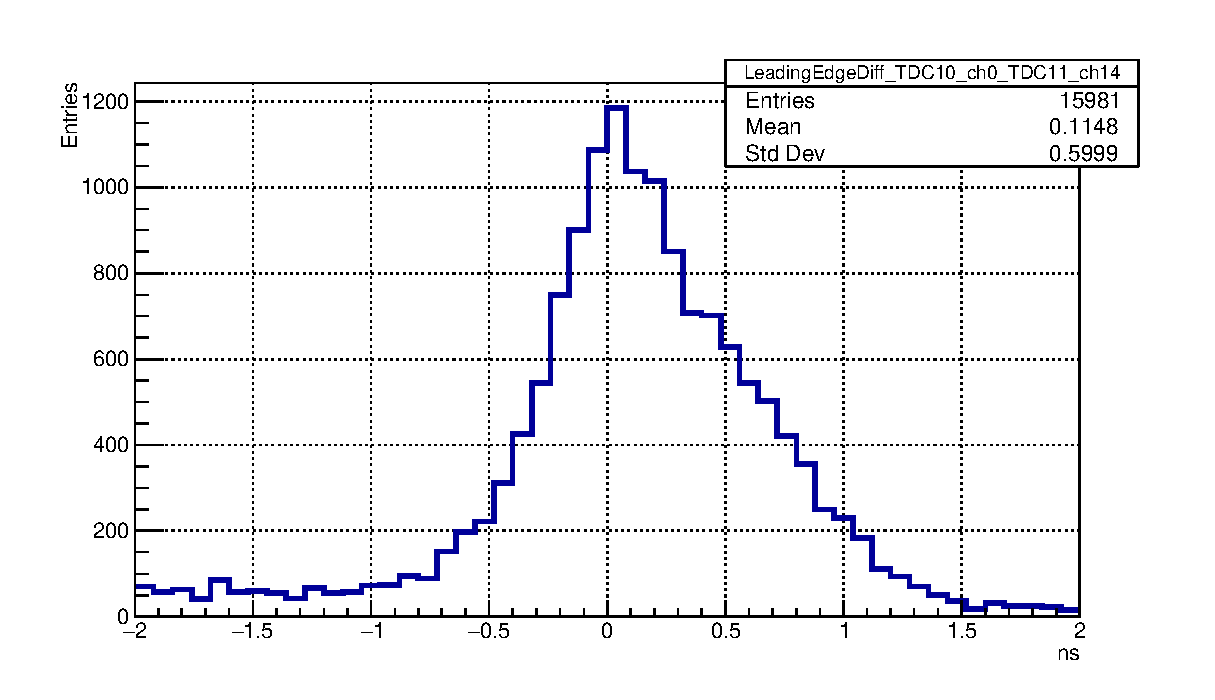
\includegraphics[width=1.0\textwidth]{pictures/LeadingEdgeDiff_TDC10_ch0_TDC11_ch14_corr.eps}
%\caption{Распределение разности временных отметок передних фронтов, соответствующих фотонам из одной вспышки лазера, зарегистрированных в заданной паре каналов, после применения калибровки точного времени и коррекции задержек.}
%\label{fig:TimeRes}
%\end{figure}

Полная ширина на полувысоте (FWHM) этого распределения составляет 750~пс, что соответствует временному разрешению 530~пс. Данное значение превосходит разброс времён прохождения сигнала в МА~ФЭУ примерно в 2~раза. Причина расхождения объясняется двумя сравнимыми вкладами: дрейфом задержек в каналах и отсутствием коррекции момента пересечения порога в зависимости от амплитуды сигнала. Для реализации такой коррекции необходимо надёжное измерение времени над порогом, что в нашем случае невозможно, см.~секцию~\ref{section:secToT}.

% Тут есть ещё такая проблема, что дефектные каналы выбрасываются и из анализа лазера, то есть там тоже фактически не 2/16/64/256 каналов, а меньше. Следовательно нужно либо приводить и то и то до отбора, либо и то и то после отбора плохих каналов.

%Кольца
%До отбора плохих каналов, но в зоне кольца / после отбора плохих каналов в зоне кольца
%TRQ = 160 каналов	/	[131]
%PMT1 = 39 каналов	/	[39]
%PMT2 = 36 каналов	/	25
%PMT5 = 41 каналов	/	36
%PMT6 = 44 каналов	/	31

%В PADIWA используется [12]-14 каналов. Я не уверен.

% Лазер
% После отбора плохих каналов /	после отбора по зоне кольца(то же самое, что и у колец)
%TRQ = 199 каналов	/	131
%PMT1 = 58 каналов	/	39
%PMT2 = 37 каналов	/	25
%PMT5 = 58 каналов	/	36
%PMT6 = 46 каналов	/	31

%В PADIWA используется [14]-16 каналов. Я не уверен.

Для того чтобы охарактеризовать временное разрешение системы в целом, помимо анализа пар каналов исследовались физически одновременные сигналы на следующих совокупностях каналов: (1)~шестнадцать каналов, считываемых одной платой PADIWA, (2)~64~канала, принадлежащих одному МА~ФЭУ, (3)~256~каналов, принадлежащих четырём соседним МА~ФЭУ. В каждом случае после коррекции задержек и калибровки точного времени, отбирались все хиты, принадлежащие одному событию, и гистограммировались разности временных отметок по всем возможным парам каналов.
Так как в анализе были отброшены дефектные каналы, а черенковское кольцо, сфокусированное на область из четырёх соседних МА~ФЭУ, проецируется лишь на часть пикселей, фактическое число каналов в случае черенковских колец отличается.
В таблице~\ref{tabl:EvolutionParams} показано, как эволюционирует среднеквадратичное отклонение и FWHM в зависимости от числа каналов. Отметим, что для событий от лазера среднеквадратичное отклонение меняется слабо, а FWHM возрастает с увеличением числа каналов, одновременно с тем, что распределение последовательно принимает форму, более близкую к распределению Гаусса. Такое поведение можно интерпретировать как размывание индивидуальных особенностей каналов в процессе усреднения. Для хитов, принадлежащих одному черенковскому кольцу (см.~\figref{fig:TimeResEvolutionRings}), и FWHM !!! и RMS !!! \textbf{Это нужно исправить?} возрастают с увеличением числа каналов, причем форма спектра характеризуется широким основанием. Вероятно, отличия между этими двумя случаями связаны с тем, что распределения фотонов во времени для черенковского кольца и вспышки лазера отличаются друг от друга.

\begin{figure}[H]
\centering
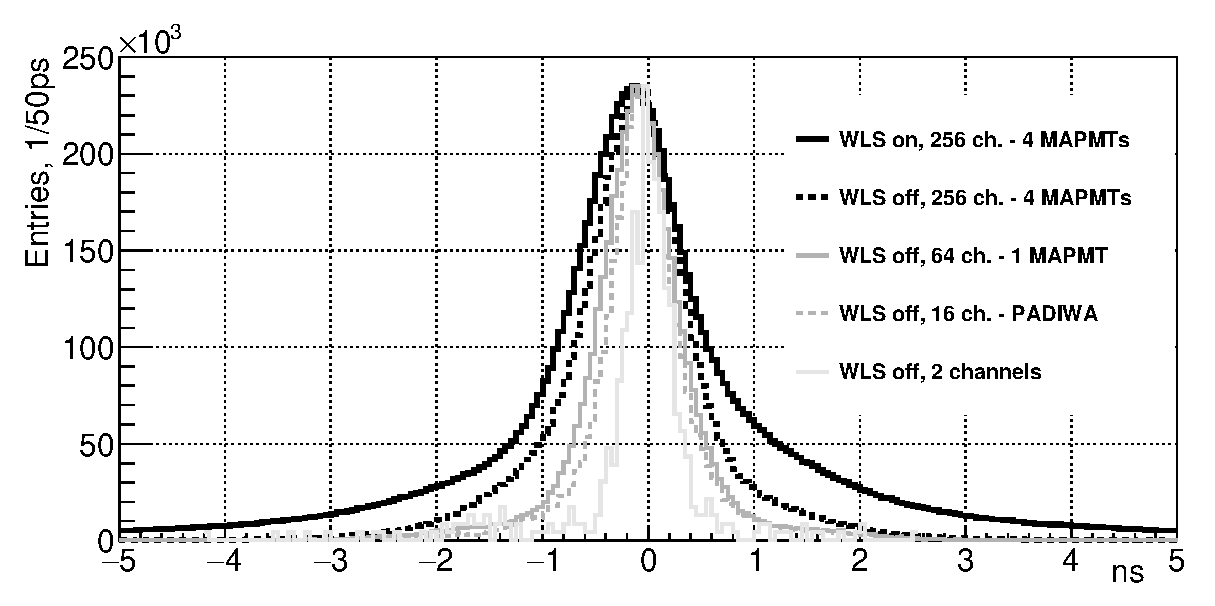
\includegraphics[width=1.0\textwidth]{pictures/Time_precision_evolution_rings_5_bw_17Mar2017.eps}
\caption{Распределения для четырёх различных наборов каналов для событий от черенковских колец. Сплошной чёрной линией показано аналогичное распределение для 4-х МА~ФЭУ со слоем сместителя спектра.}
\label{fig:TimeResEvolutionRings}
\end{figure}

%\begin{figure}[H]
%\centering
%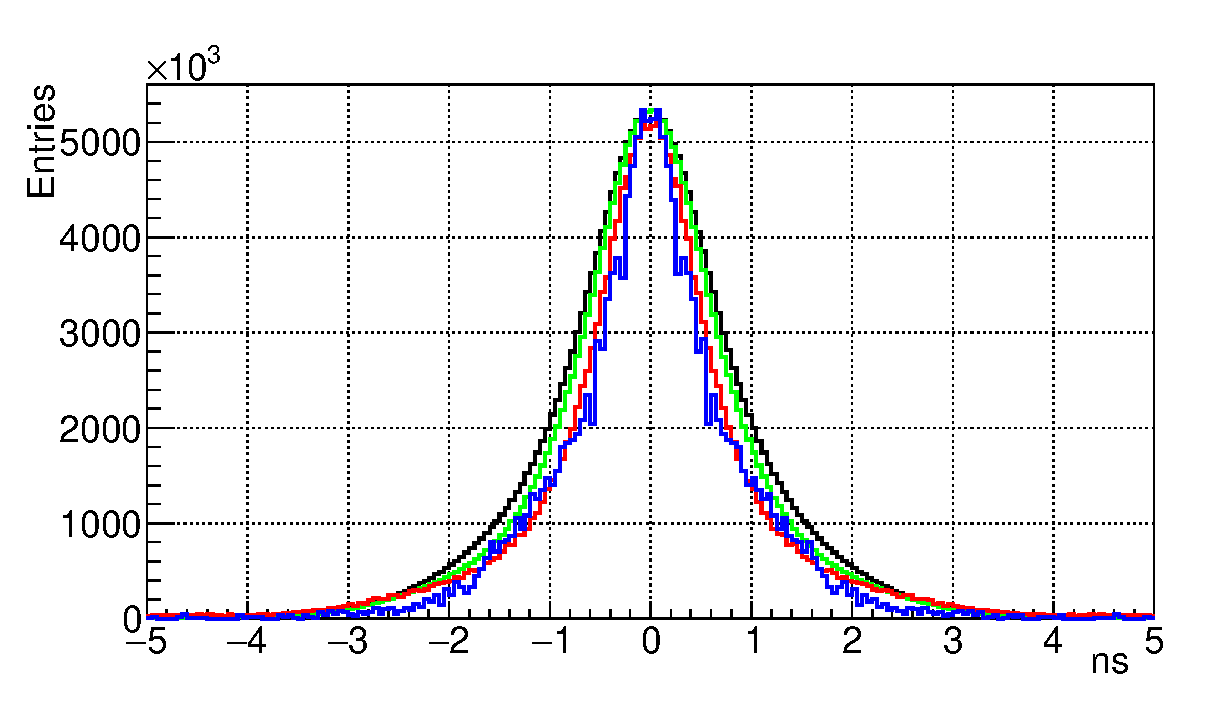
\includegraphics[width=1.0\textwidth]{pictures/24_TimePrecision_evolution_laser_feb2017.eps}
%\caption{Распределения для четырёх различных наборов каналов для событий от лазера.}
%\label{fig:TimeResEvolutionLaser}
%\end{figure}

%\begin{figure}[H]
%\centering
%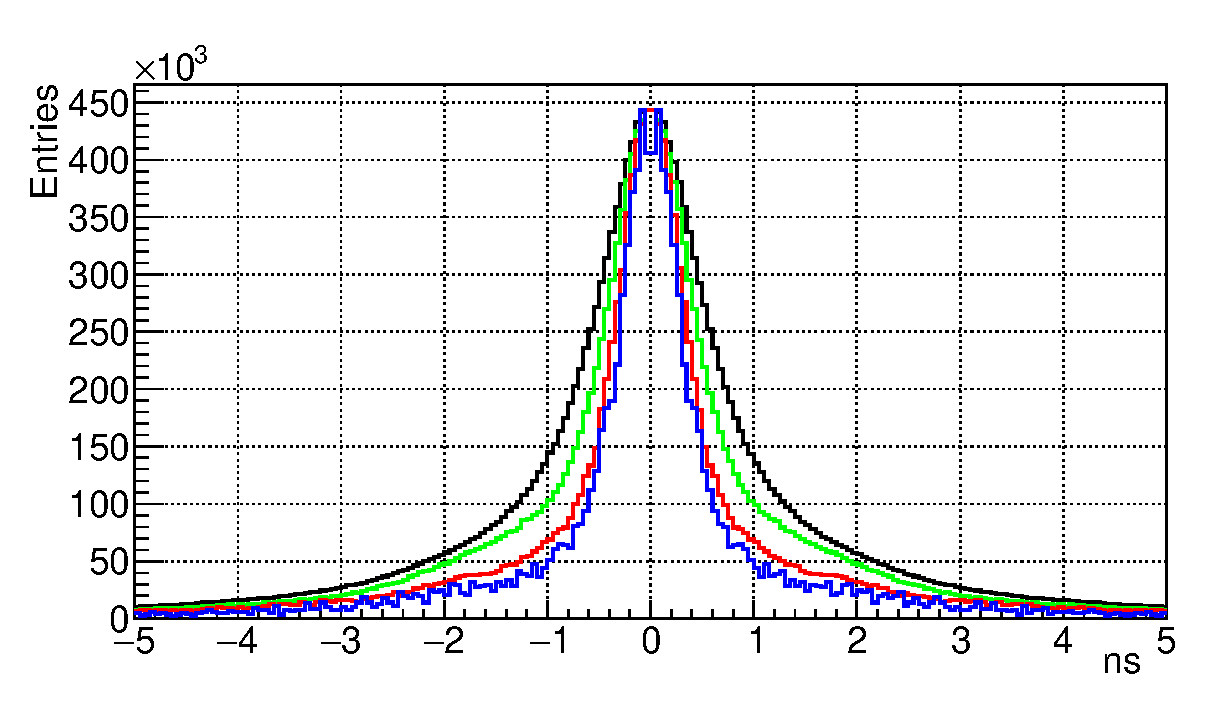
\includegraphics[width=1.0\textwidth]{pictures/25_TimePrecision_evolution_rings_feb2017.eps}
%\caption{Распределения для четырёх различных наборов каналов для событий от черенковских колец.}
%\label{fig:TimeResEvolutionRings}
%\end{figure}

\begin{table}[H]
\caption{FWHM и RMS распределений при различных наборах исследуемых каналов.}
\label{tabl:EvolutionParams}
\begin{tabular}{ | p{0.22\linewidth} | p{0.15\linewidth} | p{0.15\linewidth} | p{0.15\linewidth} | p{0.15\linewidth} | }
	\hline
	\scriptsize{Анализируемая область} & \scriptsize{Пара каналов} & \scriptsize{Плата PADIWA} & \scriptsize{Один МА~ФЭУ} & \scriptsize{Четыре МА~ФЭУ} \\
	\hline \hline
	\scriptsize{Кол-во каналов, кольца} & 2 & 14 & 39 & 160 \\
	\hline
	\scriptsize{FWHM, кольца, нс} & 0.40 & 0.60 & 0.80 & 1.05 \\
	\hline
	\scriptsize{RMS, кольца, нс} & 0.66 & 0.58 & 0.62 & 0.79 \\
	\hline \hline
	\scriptsize{FWHM, лазер, нс} & 0.7 & 1.05 & 1.30 & 1.55 \\
	\hline
	\scriptsize{RMS, лазер, нс} & 0.83 & 0.79 & 0.85 & 1.04 \\
	\hline
\end{tabular}
\end{table}
